\section{Design}
\label{sec:design}

This section presents the design of Presto by detailing
the sender, the receiver, and how the network
adapts in the case of failures and asymmetry.


%\keqiang{I put datacenter load balancing goals here, TODO: need to fix the flow later}
%
%We list the design goals of datacenter load balancing:
%\begin{enumerate}
%
%\item near-perfect traffic load balancing, uniform throughput, reduced latency (or Flow completion time), minimal packet drop rate and improved fairness, regardless of flow size
%
%\item build datacenter networks on simple, unmodified commercial Ethernet switches (versus Conga)
%
%\item traffic pattern independent load balancing (versus Conga)
%
%\item less complexity and easier to deploy, using industry proven transport layer, no modification on TCP (versus MPTCP)
%
%\item support high speed data transfer (10G or 40G+) (versus packet spraying)
%
%\item resilient to hardware or link failures, adaptive to network asymmetry (versus ECMP)
%\item support varied network topologies including: flat L2 network, L3 network or L3 Networks with L2oL3 Overlays.
%L2oL3 overlays provide both L2 adjacencies and multi-tenancy scale. Trival flat L2 network provides L2 adjacencies but not multi-tenancy scale.
%Flat L2 network with shadow MAC can prodive both L2 adjacencies and multi-tenancy scale with less configuration and management overhead.
%(On Trident II chipset based switches~\cite{trident2,smart-table,arista,cisco-nexus9000}, for 8-way multipathing, L2 network with shadow MAC scale up to 35,000 physical hosts, implying half a million VMs)
%Both L2oL3 and Flat L2 network with shadow MAC support end-host virtualization and support abtraily mapping of service and physical resources
%\end{enumerate}

%%%%%macro test - test topology, 2-tier Clos network with 8 switches and 16 hosts
\begin{figure}[!t]
        \centering
  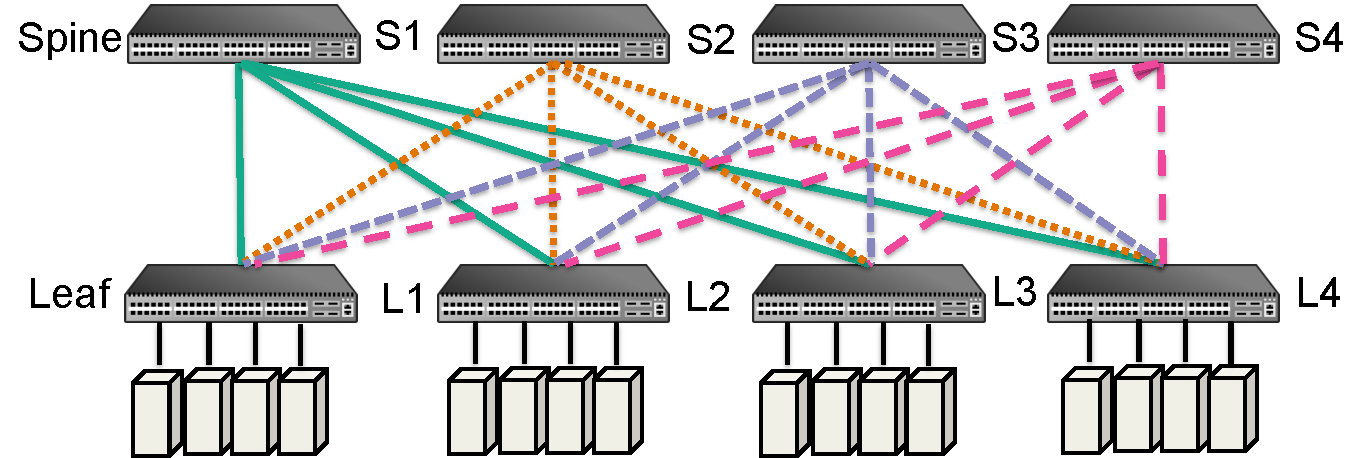
\includegraphics[width=0.45\textwidth,height=0.17\textwidth]{./figures/macro/macro_evaluation_topology_refined.pdf}
        \caption{Our testbed: 2-tier Clos network with 16 hosts.}
        \label{macro_evaluation_topology}
\end{figure}

\subsection{Sender}


\tightparagraph{Global Load Balancing at the Network Edge}
%controller allocation of paths
%installation of paths into OVS
%shadowMACs
In Presto, a centralized controller is employed to collect the
network topology and disseminate corresponding load balancing information to the edge vSwitches. 
The goal of this design is to ensure the vSwitches, as a whole, can load balance the network
in an even fashion, but without requiring an individual vSwitch to have detailed information
about the network topology, updated traffic matrices or strict coordination amongst senders.
 At a high level, the controller partitions
the network into a set of multiple spanning trees. Then, the controller
assigns each vSwitch a unique forwarding label in each spanning tree.
By having the vSwitches partition traffic over these spanning trees in a fine-grained
manner, the network can load balance traffic in a near-optimal fashion.

%We extend previous work that creates per-destination spanning trees in the network,~\ie PAST~\cite{past},
%by computing multiple disjoint spanning trees for every destination.
The process of creating spanning trees is made simple by employing multi-stage Clos
networks commonly found in datacenters. For example, in a 2-tier Clos network
with $\nu$ spine switches, the controller can easily allocate $\nu$ disjoint spanning
trees by having each spanning tree route through a unique spine switch. Figure~\ref{macro_evaluation_topology}
shows an example with four spine switches and four corresponding disjoint spanning trees.
When there are $\gamma$ links between each spine and leaf switch in a 2-tier Clos network,
the controller can allocate $\gamma$ spanning trees per spine switch.
Note that 2-tier Clos networks are scalable because they easily support a large number
of hosts with only a few high density spine switches~\cite{conga}.
In general, the controller ensures links in the network are equally covered
by the allocated spanning trees.
%~\keqiang{An example (similar to CONGA's example to convince people that 2-tier spine-leaf architecture is enough for most deployments).
%Let's use leaf switches with 48 10G ports and 12 40G uplinks. Combined with spine switches with 100s of 40G ports, 
%an non-oversubscribed 2-ter spine-leaf network which supports 20,000+ 10G nodes can be built. 
%In such a network, each 10G server can have 12 shadow MACs (there are only 12 disjoint spanning trees in the network)}

Once the spanning trees are created, the controller assigns a unique forwarding label
for each vSwitch in every spanning tree and installs them into the network.
Forwarding labels can be implemented in a variety of ways using
technologies commonly deployed to forward on labels,
such as MPLS~\cite{casado2012fabric}, VXLAN~\cite{conga,nv-mtd}, or IP encapsulation~\cite{drb}. 
In Presto,
label switching is implemented with shadow MACs~\cite{shadow-mac}. 
Shadow MACs implement label-switching for commodity Ethernet by using the 
destination MAC address as an opaque forwarding label that can easily be 
installed in L2 tables. 
Each vSwitch is assigned one shadow MAC per spanning tree.
Note Shadow MACs are extremely scalable on
existing chipsets because they utilize the large L2 forwarding table. For example,
Trident II-based switches~\cite{trident2,smart-table,arista} have 288k L2 table entries and 
thus 8-way multipathing (\ie{}, each vSwitch has 8 disjoint spanning trees)
can scale up to 36,000 physical servers.
%\eric{cite?}~\keqiang{CONGA says 20000+ is okay for an overwhelming fraction of enterprise deployments, seems to be true 
%after reading fat-tree and some googling}

%Shadow MACs allow for fine-grained, dynamic
%and consistent control of the forwarding tables in the network, but without using TCAM tables. Instead, shadow MACs use the destination MAC address
%as an opaque forwarding label in the network. Each shadow MAC can correspond to a destination-based tree. Then, the controller can preinstall
%these trees into the network. In OVS, the Presto module can use the destination IP address into a lookup table, with the entries corresponding
%to distinct paths for each destination. The OVS agent rewrites the destination MAC address to the corresponding shadow MAC address, and the Presto
%agent running on the receiver will rewrite the shadow MAC back to the original MAC address. (ugh, clean this up!). The OVS agent rewrites the destination
%MAC address of the TSO segment, and this segment is pushed to the NIC. The NIC then creates MTU-sized packets from this segment, with each packet having
%the shadow MAC address.
%
%A user space module accepts destination to multiple path mappings from the controller. Upon
%receiving a flow for the first time, the kernel module in OVS queries the user level module. If the flow is found, the path mappings are
%pushed into the kernel module. If not, the controller is queried for the destination information. OVS keeps state of the ongoing flow, and
%modifies the incoming packets with routing information for path selection as needed on a sub-flow level.



\tightparagraph{Load Balancing at the Sender}
%TSO/cell is a natural marriage
%round-robin over cells to load-balance over network
%rewrite dest MAC address to shadow MAC
% MTU size change is bad?
%chunkID insertion into packet
%make clear this is all done in OVS: blurb or two about advantages
After the controller installs the shadow MAC forwarding rules into the network, it creates a mapping
from each physical destination MAC address to a list of corresponding shadow MAC addresses. These mappings
provide a way to send traffic to a specific destination over different spanning trees. 
The mappings are pushed from the controller to each vSwitch in the network, either on-demand or preemptively.
In Presto, the vSwitch on the sender monitors outgoing traffic (\ie{}, maintains a per-flow counter in the datapath) 
and rewrites the destination MAC
address with one of the corresponding shadow MAC addresses.
The vSwitch assigns the same shadow MAC address to all consecutive segments until the 64 KB limit is reached.
In order to load balance the network effectively, the vSwitch 
iterates through destination shadow MAC addresses in a round-robin fashion. 
This allows the edge vSwitch to load balance over the network in a very fine-grained fashion.
%\eric{we have to decide where to formally define correct algorthm for chunk. that is, we don't
%load balance on TSO segments exactly, because if multiple consectutive TSO segments arrive whose sum
%is < 64 KB, then we will assign them all to the same chunk ID. this helps with small flows that consist
%of many segments, but whose sums are less than 64 KB.}
%When the first segment of a flow arrives, the vSwitch randomly chooses the a shadow MAC from
%the list and then subsequentially assigns shadow MACs to segments in a round robin fashion.

Sending each 64 KB worth of flowcells over a different path in the network can cause reordering and must
be carefully addressed.
To assist with reordering at the receiver (Presto's mechanisms for combatting reordering are detailed in the next section), 
the sender also includes a sequentially increasing {\em flowcell ID} into each segment.
For example, 
in our setup the controller installs forwarding rules solely on the destination MAC address.
ARP is handled in a centralized manner, so
the source MAC address can be used to hold the flowcell ID. Other options are possible, 
\eg{}, some schemes include load balancing metadata in the reserved bits of the VXLAN header~\cite{nvo3}.\footnote{In our
implementation, TCP options hold the flowcell ID for simplicity and ease of debugging.}
Note that since the flowcell ID and the shadow MAC address are modified before a segment is handed to the NIC,
the TSO algorithm in the NIC replicates these values to all derived MTU-sized packets.

\begin{algorithm}[t]
\caption{Pseudo-code of Presto GRO {\tt flush} function}
\label{alg:gro}
\begin{algorithmic}[1]
%\REQUIRE $n \geq 0 \vee x \neq 0$
%\ENSURE $y = x^n$
\FOR{each flow f}
\FOR{$S \in f.{\tt segment\_list}$}
%\STATE f = getFlow(S)
\IF{f.lastFlowcell == getFlowcell(S)}
\STATE f.expSeq $\leftarrow$ max(f.expSeq, S.endSeq)
\STATE pushUp(S)
\ELSIF{getFlowcell(S) $>$ f.lastFlowcell}
\IF{f.expSeq == S.startSeq}
\STATE f.lastFlowcell $\leftarrow$ getFlowcell(S)
\STATE f.expSeq $\leftarrow$ S.endSeq
\STATE pushUp(S)
\ELSIF{timeout(S)}
\STATE f.lastFlowcell $\leftarrow$ getFlowcell(S)
\STATE f.expSeq $\leftarrow$ S.endSeq
\STATE pushUp(S)
\ENDIF
\ELSE
\STATE pushUp(S)
\ENDIF
\ENDFOR
\ENDFOR
\end{algorithmic}
\end{algorithm}

\subsection{Receiver}
The main challenge at the receiver is dealing with reordering that can occur when different flowcells
are sent over different paths. The high level goal of our receiver implementation is
to mitigate the effects of the small segment flooding problem by (i) not so aggressively pushing
up segments if they cannot be merged with an incoming packet and (ii) ensuring that segments
pushed up are delivered in order.

\tightparagraph{Mitigating Small Segment Flooding} Let's use Figure~\ref{gro-break} as a motivating example 
on how to combat the small segment flooding problem. Say a polling event has occurred, and the driver retrieves
9 packets from the NIC ($P_0$-$P_8$). The driver calls the GRO handler, which tries to merge consecutive packets
into larger segments. The first three packets ($P_0$-$P_2$) are merged into a segment, call it $S_1$ (note: in practice
$S_1$ already contains in order packets received before $P_0$).
When $P_5$ arrives, a new segment $S_2$, containing $P_5$, should be created. Instead of pushing up $S_1$ (as is done currently),
both segments should be kept.
Then, when $P_3$ is received, it can be merged into $S_1$. Similarly, $P_6$ can be merged into $S_2$. This process
can continue until $P_4$ is merged into $S_1$. At this point, the gap between the original out-of-order reception ($P_2$-$P_5$)
 has been filled, and $S_1$ can be pushed up and $S_2$ can continue to grow. This means the size of the segments being pushed up is increased,
and TCP is not exposed to reordering.

The current default GRO algorithm works as follows. An interrupt by the NIC causes the driver to poll
(multiple) packets from the NIC's ring buffer. The driver calls the GRO handler on the received batch
of packets. GRO keeps a simple doubly linked list, called {\tt gro\_list}, that contains 
segments, with a flow having at most one segment in the list. When packets for a flow are
received in-order, each packet can be merged into the flow's preexisting segment. When a packet
cannot be merged, such as with reordering, the corresponding segment is pushed up (ejected from the
linked list and pushed up the networking stack) and a new segment is created from the packet. 
This process is continued until all packets in the batch are serviced. At the end 
of the polling event, a {\tt flush} function is called that pushes up all segments in the
{\tt gro\_list}.
% that are not "too new" (\ie{}, segments that were just created near the end of the polling
%event and haven't had many packets merged into them).

Our GRO algorithm makes the following high-level changes. First, multiple segments can be
kept per flow, and each flow contains a doubly linked list of its segments (called {\tt segment\_list}). 
To ensure the merging process is fast each linked list is kept in a hash table (keyed on flow).
When an incoming packet cannot be merged with any existing segment, the existing
segments are kept and a new segment is created from the packet.
New segments are added to the head of the linked list so that merging subsequent packets is typically $\mathcal{O}(1)$.
When the merging is completed over all packets in the batch, the {\tt flush} function is called. 
The {\tt flush} function decides whether to push segments up or to keep them. Segments may 
be kept so reordered packets still in flight have enough time to arrive and can then be placed in order
before being pushed up. 
Reordering can cause the linked lists to become slightly out-of-order, so
at the beginning of {\tt flush} an insertion sort is run to help easily decide if segments are in order.
%\eric{this is likely too long and too repetitive with section 2. keqiang, please go over to check for
%correctness. we need to figure out the write level of detail to go into here. we also need
%to say what the impact of using sMACs is here... how are flows decided? i'm also missing
%other pushUp events: like max segment size being reached, timeout occuring on segment, etc.}

The pseudo-code of our {\tt flush} function is presented in Algorithm~\ref{alg:gro}.
For each flow, our algorithm keeps track of the next expected in-order
sequence number ({\tt f.expSeq}) and the corresponding flowcell ID
of the most recently received in-order sequence number ({\tt f.lastFlowcell}).
The {\tt flush} function iterates over 
the sorted segments ($S$), from lowest sequence number to highest sequence number, in the {\tt segment\_list} (line 2).
The rest of the code is presented in the subsections that follow.


\tightparagraph{How to Differentiate Loss from Reordering?} 
In the case of no loss or reordering, our algorithm keeps pushing up segments and updating state. Lines 3-5
deal with segments from the same flowcell ID, so we just need to update {\tt f.expSeq} each time. Lines 
6-10 represent the case when the current flowcell ID is fully received and we start to receive the
next flowcell ID. The problem, however, is when there is 
a gap that appears between the sequence numbers of the segments. When a gap is encountered,
it isn't clear if it is caused from reordering or from loss. If the gap is due to reordering,
our algorithm should be conservative and try to wait to receive the packets that "fill in the gap" 
before pushing segments up to TCP. If the gap is due to loss, however, then we should push up the 
segments immediately so that TCP can react to the loss as quickly as possible.

%We solve this seemingly difficult problem in a simple fashion. 
%Since chunk sizes are small and 
%all packets within a chunk are routed on the same shadow MAC address, it is highly likely all packets
%within the same chunk will traverse the same network path
To solve this problem, we leverage the fact that all packets carrying the same flowcell ID traverse the 
same path and should be in order.
This means incoming sequence numbers can be monitored to check for
gaps. A sequence number gap within the same flowcell ID is assumed to be a loss, and not reordering,
so those packets are pushed up immediately (lines 3-5).
Note that because a flowcell consists of many packets (a 64KB flowcell consists
of roughly 42 1500 byte packets), when there is a loss, it is likely that it occurs within flowcell boundaries. 
The corner case, when a gap occurs on the flowcell boundary, leads us to the next design question.

\tightparagraph{How to Handle Gaps at Flowcell Boundaries?}
When a gap is detected in sequence numbers at flowcell boundaries, it is not clear if the gap is due
to loss or reordering. Therefore, the segment should be held long enough to
handle reasonable amounts of reordering, but not so long that TCP cannot respond
to loss promptly. Previous approaches that deal with reordering typically employ a large static
timeout (10ms)~\cite{drb}. 
Setting the timeout artificially high can handle reordering, but hinders TCP when the gap is
due to loss. 
Setting a lower timeout is difficult because it depends on many dynamic factors such as delays between
segments at the sender, amount of network congestion in different paths, and traffic patterns (multiple flows 
received at the same NIC affect inter-arrival time). 
%because there are often many causes for variations in delay: 
%the sender (senders often have delays between segments), the network (different
%queue lengths from congestion over different paths), and the traffic patterns (multiple flows received at the same NIC affect
%inter-arrival time). 
%As a result, we devised an adaptive timeout to help deal with dynamic variations. 
As a result, we devise an adaptive timeout scheme, which monitors recent reordering events and sets a dynamic timeout value accordingly.
Presto tracks cases when there is reordering, but no loss, on flowcell boundaries and keeps an exponentially-weighted
moving average ($EWMA$) over these times. Presto then applies a timeout of $\alpha * EWMA$ to a segment when a gap is 
detected on flowcell boundaries. 
Here $\alpha$ is an empirical parameter that allows for timeouts to grow. As a further optimization, if a segment
has timed out, but a packet has been merged into that segment in the last $\frac{1}{\beta} * EWMA$ time interval, then 
the segment is still held in hopes of preventing reordering. We find $\alpha$ and $\beta$
work over a wide range of parameters and set both of them to 2 in our experiments. A timeout firing is dealt with in lines 11-15.
%\eric{take out GRO\_LIST.full()?}

%\tightparagraph{How to handle shadow MACs with OVS?}
%~\keqiang{Can we take this paragraph out, just feel that it breaks the flow of this paper}
%OVS has many optimizations to handle segments at line rate. One problem with using shadow MACs is that many keys 
%may be created for the same flow (since OVS hashes on MAC addresses).
%At the receiver, we overwrite the destination MAC address to the physical MAC address and overwrite the source MAC 
%address to a consistent dummy value\footnote{The controller handles all ARP messages in Presto} before any lookups. At the sender,
%we do not overwrite any MAC address until after the table lookup.
%Rewriting the MAC address also makes any of our changes completly transparent to higher layers in the networking
%stack.
%\eric{move to discussion?}

%We found OVS makes a few assumptions in which our code caused issues. The default implementation of OVS does a flow
%lookup in which it uses hashed header values as a key. The key hashes on ethernet addresses, and the first time a packet is received
%for this tuple, OVS must do a lookup into user level. In the implementation, the first packet received is pushed to user
%level, but the packet size is bound to 1500 bytes. This means if a large packet is received as the first packet on a key,
%then OVS must break the large packet into 1500 byte packets and pushes them {\em all} to user space. Normally, this is not a problem,
%because the SYN packet is a first packet of a flow, so (i) it is small and (ii) the round-trip time of TCP's handshake gives
%the user level calls time to complete. In Presto however, the SYN packet may not share the same ethernet destination as subsequent
%data packets. This means that a large data packet can be the first packet to arrive over a given ethernet destination. This
%originally caused substainal packet reordering and much overhead at the beginning of a TCP connection in Presto. We were able
%to simply fix the problem by writing the shadow MAC address back to the original destination MAC address before any key lookups
%in OVS. Rewriting the shadow MAC address also makes any of our changes completly transparent to higher layers in the networking
%stack.

%\eric{should we talk about using a path ID instead of a chunk ID? then don't have to change anything but shadowMAC. this 
%is only doable if the receiver knows the round-robin scheduling that the sender is employing. should we also talk
%about using something like source port to get ECMP to hash onto different paths? this is done by MPTCP and the 
%vmware blog}


\subsection{Failure Handling and Asymmetry}
%Monthly switch and link availability have been 
%shown to be 99.99\% and 99.95\%, respectively~\cite{wcmp}.
When failures occur, Presto relies on the controller to update the forwarding
behavior of the affected vSwitches. The controller can simply prune the spanning
trees that are affected by the failure, or more generally enforce a weighted
scheduling algorithm over the spanning trees.
Weighting allows for Presto to evenly distribute traffic over an asymmetric topology.
Path weights can be implemented in a simple fashion by duplicating shadow MACs used in
the vSwitch's round robin scheduling algorithm.
For example, assume we have three paths in total ($p_1$, $p_2$ and $p_3$) and their updated weights are 0.25, 0.5 and 0.25 respectively.
Then the controller can send the sequence of $p_1$, $p_2$, $p_3$, $p_2$ to the vSwitch, which
can then schedule traffic over this sequence in a round robin fashion to realize the new path weights.
This way of approximating path weights in the face of network
asymmetry is similar to WCMP~\cite{wcmp}, but instead of having to change switch firmware and use
scarce on-chip SRAM/TCAM entries, we can push the weighted load balancing entirely to the network edge.

As an added optimization, Presto can leverage any fast failover features that 
the network supports, such as BGP fast external failover, MPLS fast reroute, or OpenFlow failover groups. Fast failover detects port failure and can move corresponding traffic
to a predetermined backup port.\footnote{Hardware failover latency ranges from several to tens of milliseconds~\cite{ipblog-failover,huawei-failover}}
This ensures traffic is moved away from the failure rapidly and the network
remains connected when redundant links are available.
% and contains redundant links~\keqiang{like Facebook's "protection ring"~\cite{farrington2013facebook}}. 
Moving to backup links causes imbalance in the network,
so Presto relies on the controller learning of the network change, computing weighted multipath schedules, and
disseminating the schedules to the vSwitches. 

%\subsection{Non-SDN Environments}
%Instead of using shadow MACs, Presto can be implemented in non-SDN environments in the following manner. First,
%the approach must rely on ECMP in the fabric. ECMP can be configured to hash on a wide variety of network headers (cite).
%As done in MPTCP, and mentioned in online discussions, the Layer 4 source port can be varied to force ECMP to 
%route different sub-flows onto different paths. In Presto, the chunk ID can easily be stashed in the TCP source
%port. HOW DOES THE RECEIVER DEAL WITH THIS? (must not break RSS, must allow receiver to echo packets back to sender, etc). 

%
% old stuff.
%
%PAST~\cite{past}.
%Open vSwitch has been acting as the intelligent {\em network edge} in datacenter networks~\cite{ovs-extending,ovs-edge,nv-mtd}.
%TCP offload~\cite{tcp-offload,optimize-tcp-receive}.
%Generic Receive Offload (GRO)~\cite{gro,bullettrains}.
%New API (NAPI)~\cite{understanding-linux-network}.
%Link/switch failures in datacenters~\cite{dc-failures,wcmp}.
